As part of a study of its sheet metal assembly process, a major automobile manufacturer
uses sensors that record the deviation from the nominal thickness (millimeters) at six locations
on a car. The first four are measured when the car body is complete and the last two
are measured on the underbody at an earlier stage of assembly. Data on 50 cars are
given in Table 5.14.
\begin{enumerate}[label= (\alph*)]
    \item The process seems stable for the first 30 cases. Use these cases to estimate \textbf{S} and $\bar{\textbf{x}}$.
    Then construct a $T^{2}$ chart using all of the variables. Include all 50 cases.

    \begin{figure}[H]
        \centering
        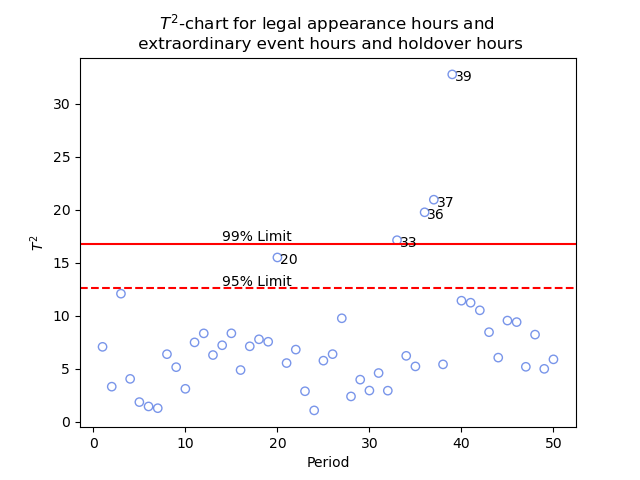
\includegraphics[scale=0.65]{./python/chapter-5/Question-5-28-a-T2.png}
    \end{figure}

    \item Which individual locations seem to show a cause for concern?
    
    There are five cases that exceed our 95\% limit (20, 33, 36, 37, 38, 39), four of which also exceed the 99\% limit (33, 36, 37, 38, 39).

    \begin{NiceTabular}{|ccccccc|c|}
        \hline
        Index &    x1 &    x2 &    x3 &    x4 &   x5 &    x6 & $T^{2}$ \\
        \hline
        20    & -0.46 &  0.36 &  0.24 & -0.58 & 0.15 &  0.25 & 15.50 \\
        33    & -0.47 & -0.16 & -0.34 & -0.31 & 0.85 &  0.60 & 17.13 \\
        36    & -0.90 & -0.40 &  0.75 & -0.31 & 0.60 & -0.10 & 19.76 \\
        37    & -0.50 & -0.35 &  0.84 & -0.52 & 0.35 & -0.75 & 20.95 \\
        39    & -0.60 & -0.35 & -0.35 & -0.34 & 0.60 &  0.85 & 32.76\\
        \hline
    \end{NiceTabular}

\end{enumerate}